\chapter{Spherically symmetric average model}
\label{chapter:1Dmodel}

In this appendix we determine the spherically symmetric (radial) average of model GLAD-M25.
To accomplish this,
we first need to transform the 3D spectral-element mesh --- which includes ellipticity, topography/bathymetry and undulations on internal boundaries --- into a spherical volume.
After these adjustments, we obtain a spectral-element mesh for a perfect cubed sphere~\cite{KoTr02a}.

In the spherical mesh, the model may be expressed in the form
\begin{equation}
    m(\mathbf{x})=\sum_{\mathrm{elem}}\sum_{\alpha,\beta,\gamma}m^{\alpha\beta\gamma}\,h_{\alpha}(\xi)\,h_{\beta}(\eta)\,h_{\gamma}(\zeta)\,
    \quad ,
\end{equation}
where~$h_\alpha$ denotes a Lagrange polynomial, and where we have used the invertible mapping
\begin{equation}
    \mathbf{x}=\mathbf{x}(\xi,\eta,\zeta)
\end{equation}
between spatial points~$\mathbf{x}=\{x,y,z\}$ and Gauss-Lobatto-Legendre (GLL) points in the reference element~$\{\xi,\eta,\zeta\}$~\cite{KoTr99}.

The spherically symmetric part of the model is defined as
\begin{equation}
    \overline{m}(r)=\frac{1}{4\pi}\,\int_\Omega m(\mathbf{x})\,\mathrm{d} \Omega
    \quad,
\end{equation}
where~$r$ denotes the radius and~$\Omega$ the unit sphere.

Using 2D GLL quadrature~\cite{KoTr99} in the unit sphere,
the radial average may be determined numerically via GLL quadrature:
\begin{equation}
    \overline{m}(r)=\frac{1}{4\pi\,r^2}\,\sum_{\alpha,\beta}\omega_\alpha\omega_\beta\,m^{\alpha\beta}(r)\,J^{\alpha\beta}(r)
    \quad.
    \label{eq:radial_average}
\end{equation}
Here~$\alpha$ and~$\beta$ denote GLL points in the sphere with radius~$r$\,,
$\omega_\alpha$ denotes a GLL quadrature weight, and $J^{\alpha\beta}(r)$ is the 2D Jacobian of the mapping to the sphere.
%It is important to carry out the summations in~(\ref{eq:radial_average}) at the elemental level to ensure that first-order discontinuities are honored in the process.

Figure~\ref{fig:global-average} shows the resulting radial averages of the isotropic shear and compressional wavespeeds for model~GLAD-M25
compared to 1D starting model~STW105~\cite{kustowski2008anisotropic} and PREM~\cite{PREM}.
The radial average of~GLAD-M25 remains very close to the radial starting model~STW105.
The main difference between these two models and~PREM
is the absence of the 220~km discontinuity and a lower~$V_\text{P}/V_\text{S}$ ratio in the top 200~km.

\begin{figure}
  \centering
  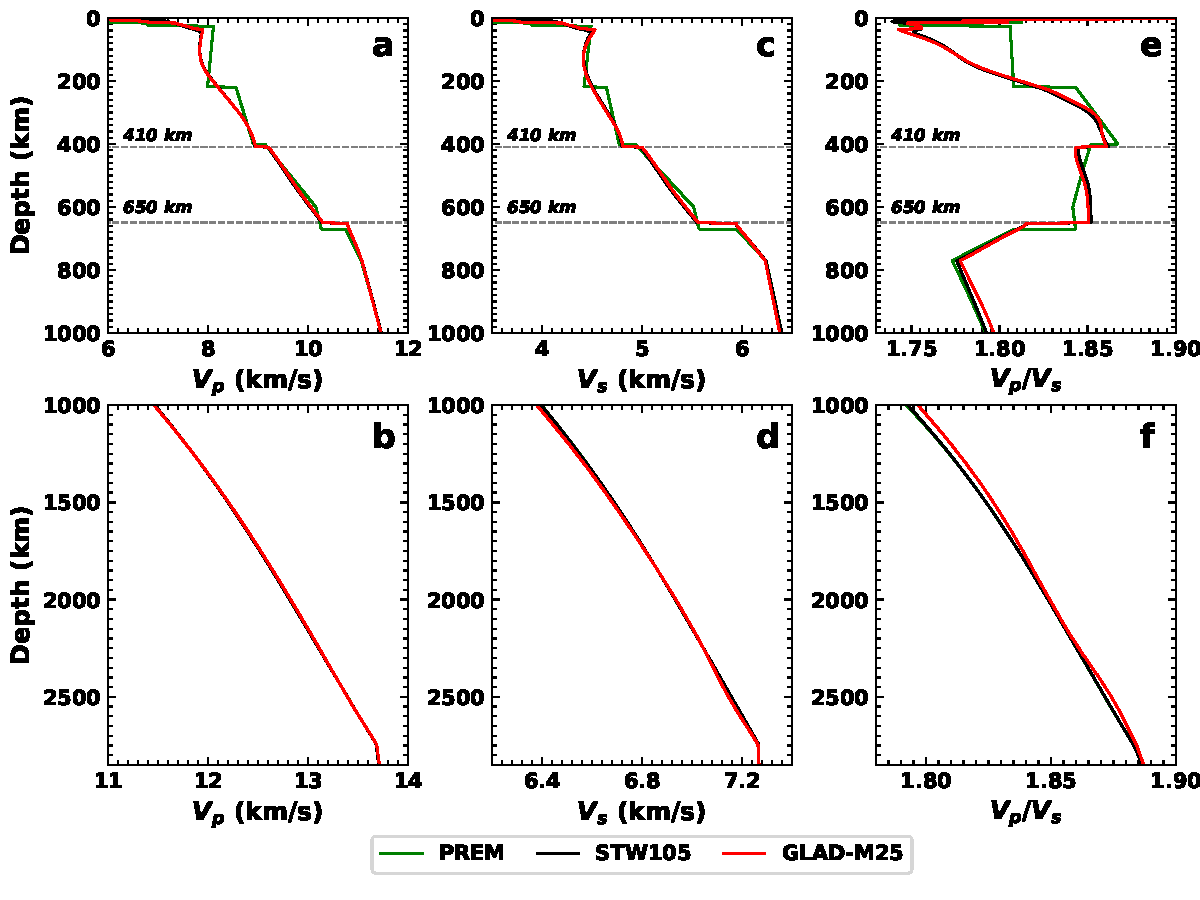
\includegraphics[width=0.8\textwidth]{ch-GLADM25/figures/1d_profile.pdf}
  \caption[1D radial shear and compressional wavespeed profiles for GLAD-M25, STW105, and PREM]
  {\small{1D radial shear and compressional wavespeed profiles for GLAD-M25, STW105, and PREM.
  The reference frequency for physical dispersion is ~7.77~mHz.}}
  \label{fig:global-average}
\end{figure}

\begin{figure}
  \centering
  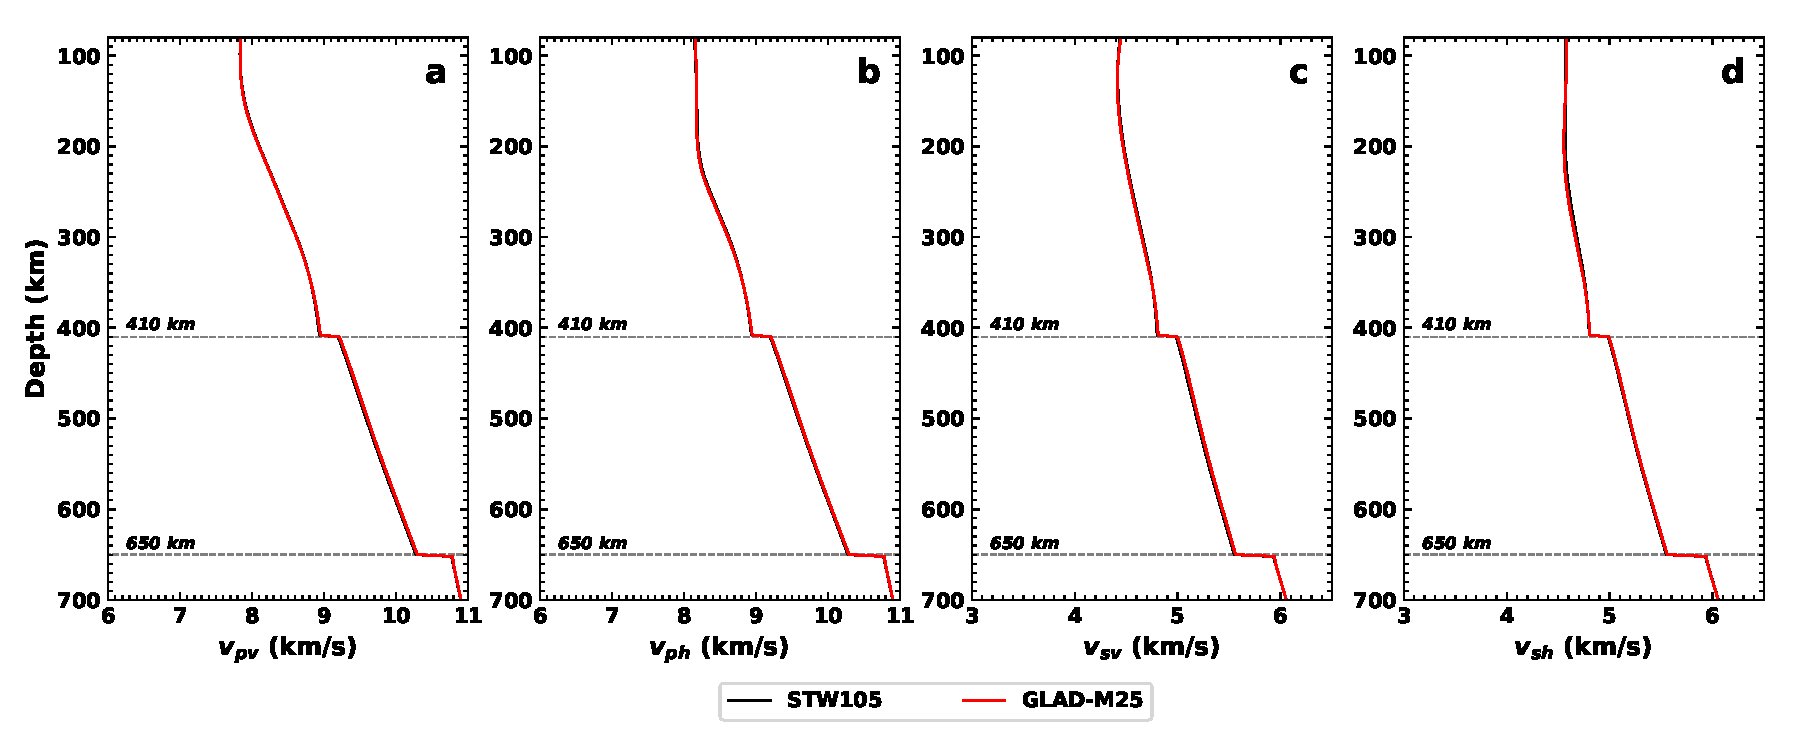
\includegraphics[width=0.9\textwidth]{ch-GLADM25/figures/1d_profile_ra.pdf}
  \caption[1D radial-anisotropic shear and compressional wavespeed profiles for GLAD-M25 and STW105]
  {\small{1D radial-anisotropic shear and compressional wavespeed profiles for GLAD-M25 and STW105. The reference frequency for physical dispersion is ~7.77~mHz.}}
  \label{fig:global-ra-average}
\end{figure}

\chapter{Spherical harmonic model expansion}
\label{chapter:shanalysis}

In this appendix we express model GLAD-M25 in a spherical harmonic basis
to facilitate easy plotting, analysis, and comparisons with other models.
The resulting spherical harmonic model should only be used for these purposes, not for numerical simulations, which should always be based on the fully 3D spectral-element mesh.

To accomplish the transformation,
we first need to transform the 3D mesh --- which includes ellipticity, topography/bathymetry and undulations on internal boundaries --- into a spherical volume.
After these adjustments, we obtain a spectral element mesh for a perfect sphere,
that is, the sort of mesh used for spherically symmetric earth models, such as PREM~\cite{PREM}.

In the spherical mesh, the model may be expressed in the form
\begin{equation}
    m(\mathbf{x})=\sum_{\mathrm{elem}}\sum_{\alpha,\beta,\gamma}m^{\alpha\beta\gamma}\,h_{\alpha}(\xi)\,h_{\beta}(\eta)\,h_{\gamma}(\zeta)\,
    \quad ,
\end{equation}
where~$h_\alpha$ denotes a Lagrange polynomial, and where we have used the invertible mapping
\begin{equation}
    \mathbf{x}=\mathbf{x}(\xi,\eta,\zeta)
    \label{eq:map}
\end{equation}
between spatial points~$\mathbf{x}=\{x,y,z\}$ and Gauss-Lobatto-Legendre (GLL) points in the reference element~$\{\xi,\eta,\zeta\}$~\cite{KoTr99}.

Our goal is to expand our spectral-element model in a spherical harmonic basis, i.e.,
\begin{equation}
    m(\mathbf{x})=\sum_{n=0}^N\sum_{\ell = 0}^L\sum_{m=-\ell}^\ell {}_nC_{\ell m}\,R_n(r)\,Y_{\ell m}(\theta,\phi)
    \quad ,
    \label{eq:m}
\end{equation}
where~$r$ denotes the radius, $\theta$ colatitude, and~$\phi$ longitude.
We choose a radial basis of the form~$R_n(r)$\,, $n=0,\ldots,N$\,,
e.g., layers or B-splines.
These radial basis functions need to be chosen sufficiently dense to mimic the density of the radial spectral element mesh.
The radial basis may or may not be orthogonal,
i.e.,
\begin{equation}
    \int_b^a R_{n'}(r)\,R_{n}(r)\,r^2\mathrm{d}r = A_{n'n}
    \quad ,
    \label{eq:R}
\end{equation}
where~$b$ denotes the radius of the CMB and~$a$ the free surface.
The matrix elements~$A_{n'n}$ define a positive definite matrix which is invertible.
As lateral basis functions we use fully normalized spherical harmonics~$Y_{\ell m}(\theta,\phi)$\,, $\ell=0,\ldots,L$ and $m=\mbox{}-\ell,\ldots,\ell$\,, i.e.,~\cite{DT98}
\begin{equation}
    \int_0^{2\pi}\int_0^\pi Y^*_{\ell'm'}(\theta,\phi)\,Y_{\ell m}(\theta,\phi)\,\sin\theta\,\mathrm{d}\theta\,\mathrm{d}\phi = \delta_{\ell' \ell}\,\delta_{m'm}
    \quad ,
    \label{eq:Y}
\end{equation}
where an asterisk denotes complex conjugation.
The maximum degree~$L$ needs to be chosen to resolve the spectral-element mesh laterally.

To obtain the expansion coefficients~${}_nC_{\ell m}$\,, we multiply Eqn.~(\ref{eq:m}) by
$R_{n'}(r)\,Y^*_{\ell' m'}(\theta,\phi)$ and integrate over the volume of the mantle and crust,~$V$\,, using Eqns.~(\ref{eq:R} and~(\ref{eq:Y}):
\begin{equation}
    \int_V m(\mathbf{x})\,R_{n'}(r)\,Y^*_{\ell' m'}(\theta,\phi)\,\mathrm{d}^3\mathbf{x}=\sum_{n=0}^N {}_nC_{\ell' m'}\,A_{n'n}
    \quad ,
\end{equation}
We evaluate the integral on the left using GLL quadrature~\cite{KoTr99}:
\begin{equation}
    \sum_{\mathrm{elem}}\sum_{\alpha,\beta,\gamma}\omega_\alpha\,\omega_\beta\,\omega_\gamma\,m^{\alpha\beta\gamma}\,J^{\alpha\beta\gamma}\,R_{n'}^{\alpha\beta\gamma}\,Y_{\ell'm'}^{*\,\alpha\beta\gamma}
    =\sum_{n=0}^N {}_nC_{\ell' m'}\,A_{n'n}
    \quad .
\end{equation}
Here~$\omega_\alpha$ denotes a GLL quadrature weight,
$J_{\alpha\beta\gamma}$ the Jacobian of the mapping~(\ref{eq:map}) evaluated on the GLL points,
and $R_{n'}^{\alpha\beta\gamma}$ and $Y_{\ell'm'}^{*\,\alpha\beta\gamma}$ the values of the radial and spherical harmonic basis functions at a GLL point.

Finally, the desired model coefficients may be obtained ---one combination of $n$\,, $\ell$\,, and $m$ at a time--- via
\begin{equation}
    {}_nC_{\ell m}=\sum_{n'}A^{-1}_{nn'}\sum_{\mathrm{elem}}\sum_{\alpha,\beta,\gamma}\omega_\alpha\,\omega_\beta\,\omega_\gamma\,m^{\alpha\beta\gamma}\,J^{\alpha\beta\gamma}\,R_{n'}^{\alpha\beta\gamma}\,Y_{\ell m}^{*\,\alpha\beta\gamma}
    \quad ,
    \label{eq:Cnlm}
\end{equation}
where~$A^{-1}$ denotes the inverse of the~$N\times N$ matrix~$A$.
Expressions of the form~(\ref{eq:Cnlm}) are commonplace in spectral-element simulations,
and thus easily calculated.

The normalized power per degree~$\ell$ may be calculated via
\begin{equation}
    \sigma_\ell^2=\frac{1}{2\ell+1}\,
    \sum_{n' = 0}^N\sum_{n = 0}^N\sum_{m = -\ell}^\ell\,A_{n'n}\,{}_{n'}C^*_{\ell m}\,{}_{n}C_{\ell m}
    \quad .
\end{equation}
Alternatively,
one may wish to calculate the power per degree as a function of radius,
which is determined via
\begin{equation}
    \Sigma_\ell^2(r)=\frac{1}{2\ell+1}\,
    \sum_{n' = 0}^N\sum_{n = 0}^N\sum_{m = -\ell}^\ell\,R_{n'}(r)\,R_{n}(r)\,{}_{n'}C^*_{\ell m}\,{}_{n}C_{\ell m}
    \quad .
\end{equation}

Instead of the complex spherical harmonic model expansion~(\ref{eq:m}),
we may wish to use a real spherical harmonic expansion of the form~\cite{DT98}
\begin{equation}
\begin{split}
    m(\mathbf{x}) \ = & \ \sum_{n=0}^N\sum_{\ell = 0}^L \left[ {}_na_{\ell 0}\,R_n(r)\,X_{\ell 0}(\theta)
   +\sqrt{2}\sum_{m=1}^\ell R_n(r)\,({}_na_{\ell m}\,\cos m\phi+{}_nb_{\ell m}\,\sin m\phi)\,X_{\ell m}(\theta)\right]
    \quad ,
\end{split}
    \label{eq:mreal}
\end{equation}
where Eqn.~B.30~\cite{DT98}
\begin{equation}
    Y_{\ell m}(\theta,\phi)=X_{\ell m}(\theta)\exp(i m\phi)
    \quad ,
\end{equation}
and where
\begin{equation}
    {}_na_{\ell 0}=\sum_{n'}A^{-1}_{nn'}\sum_{\mathrm{elem}}\sum_{\alpha,\beta,\gamma}\omega_\alpha\,\omega_\beta\,\omega_\gamma\,m^{\alpha\beta\gamma}\,J^{\alpha\beta\gamma}\,R_{n'}^{\alpha\beta\gamma}\,X_{\ell m}^{\alpha\beta\gamma}
    \quad ,
\end{equation}
and for~$1\le m\le \ell$
\begin{equation}
    {}_na_{\ell m}=\sqrt{2}\,\sum_{n'}A^{-1}_{nn'}\sum_{\mathrm{elem}}\sum_{\alpha,\beta,\gamma}\omega_\alpha\,\omega_\beta\,\omega_\gamma\,m^{\alpha\beta\gamma}\,J^{\alpha\beta\gamma}\,R_{n'}^{\alpha\beta\gamma}\,X_{\ell m}^{\alpha\beta\gamma}\,(\cos m \phi)^{\alpha\beta\gamma}
    \quad ,
\end{equation}
\begin{equation}
    {}_nb_{\ell m}=\sqrt{2}\,\sum_{n'}A^{-1}_{nn'}\sum_{\mathrm{elem}}\sum_{\alpha,\beta,\gamma}\omega_\alpha\,\omega_\beta\,\omega_\gamma\,m^{\alpha\beta\gamma}\,J^{\alpha\beta\gamma}\,R_{n'}^{\alpha\beta\gamma}\,X_{\ell m}^{\alpha\beta\gamma}\,(\sin m \phi)^{\alpha\beta\gamma}
    \quad .
\end{equation}
The normalized power per degree~$\ell$ may then be calculated via
\begin{equation}
    \sigma_\ell^2=\frac{1}{2\ell+1}\,\sum_{n'=0}^N\,\sum_{n=0}^N\,A_{n'n}\,\left[{}_{n'}a_{\ell 0}\,{}_{n}a_{\ell 0}+\sum_{m=1}^\ell({}_{n'}a_{\ell m}\,{}_na_{\ell m}+{}_{n'}b_{\ell m}\,{}_nb_{\ell m})\right]
    \quad ,
    \label{eq:powerdegree}
\end{equation}
and the normalized power per degree as a function of radius is determined via
\begin{equation}
    \Sigma_\ell^2(r)=\frac{1}{2\ell+1}\,\sum_{n'=0}^N\,\sum_{n=0}^N\,R_{n'}(r)\,R_{n}(r)\,\left[{}_{n'}a_{\ell 0}\,{}_{n}a_{\ell 0}+\sum_{m=1}^\ell({}_{n'}a_{\ell m}\,{}_na_{\ell m}+{}_{n'}b_{\ell m}\,{}_nb_{\ell m})\right]
    \quad .
    \label{eq:powerdegreeradius}
\end{equation}
In Fig.~\ref{fig:powerspectra} we plot the normalized power per degree~$\ell$ for models S362ANI, GLAD-M15, and GLAD-M25,
and Fig.~\ref{fig:powerspectraradius} shows the normalized power per degree as a function of radius
for the same set of models.

\begin{figure}
  \centering
  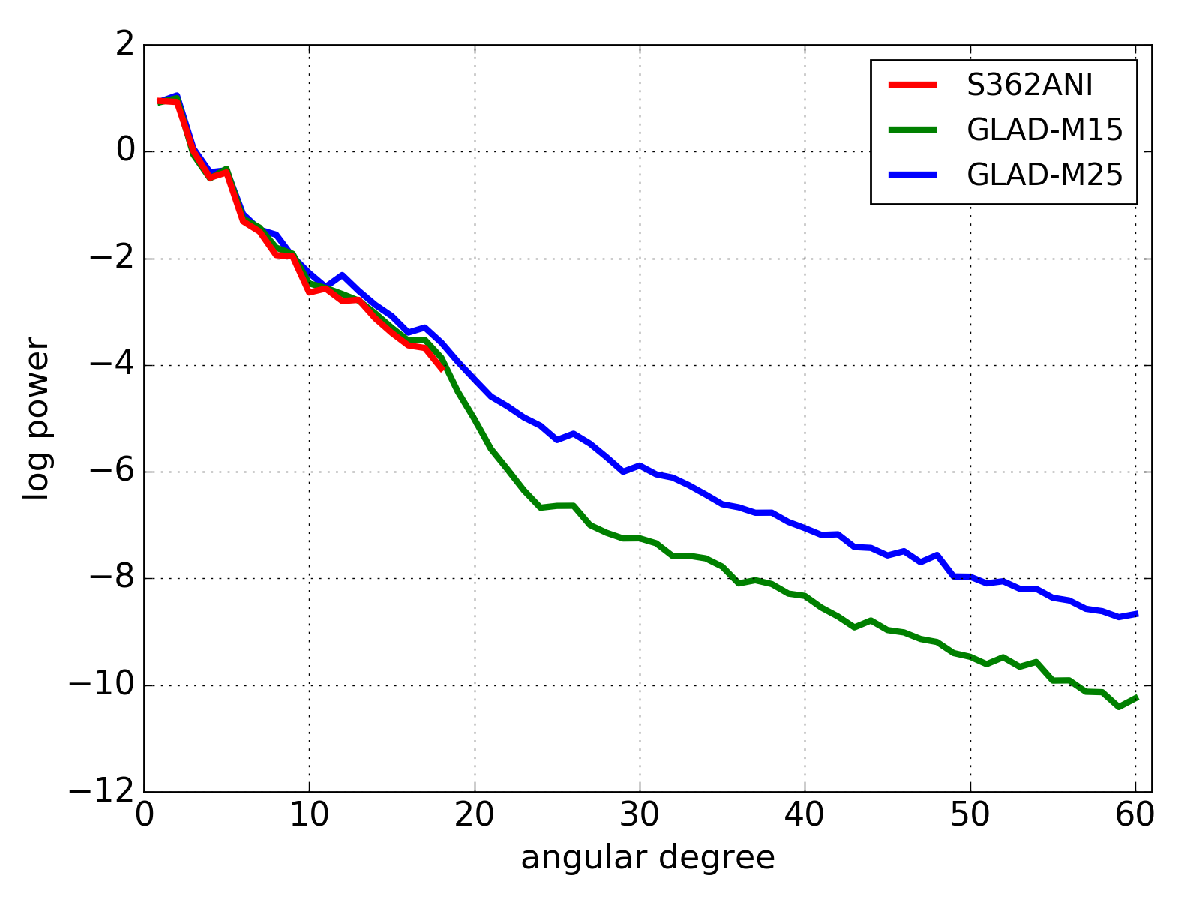
\includegraphics[width=0.5\textwidth]{ch-GLADM25/figures/power.pdf}
  \caption[Normalized power per degree~$\ell$,]{\small{Normalized power per degree~$\ell$, based on Eqn.~(\ref{eq:powerdegree}), for models S362ANI (red), GLAD-M15 (green), and GLAD-M25 (blue).
  The calculation includes depths greater than 120~km.
  Model S362ANI has no power beyond degree~18,
  and model S40RTS has no power beyond degree~40.
  (Courtesy of Caio Ciardelli.)
  }}
  \label{fig:powerspectra}
\end{figure}
